\documentclass[crop,border={0pt 0 0 0},tikz]{standalone}
\usetikzlibrary{backgrounds,decorations.markings}
\tikzset{>=latex}
\tikzset{->-/.style={decoration={
  markings,
  mark=at position .5 with {\arrow{>}}},postaction={decorate}}}
\begin{document}
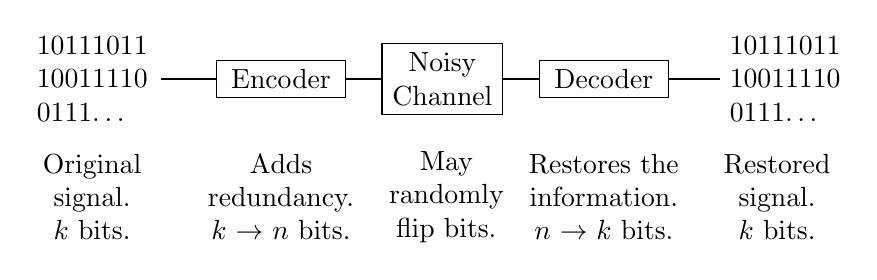
\begin{tikzpicture}
    \node[anchor=west, text width=1.4cm] at (-1.7,0) {10111011 \\ 10011110 \\ 0111\dots};
    \draw[black] (0,0) -- (7.1,0);
    \node[draw,fill=white,anchor=west,text width=1.4cm, align=center] at (0.7,0) {Encoder};
    \node[draw,fill=white,anchor=west, text width=1.3cm, align=center] at (2.8,0) {Noisy Channel};
    \node[draw,fill=white,anchor=west,text width=1.4cm, align=center] at (4.8,0) {Decoder};
    \node[anchor=west, text width=1.4cm] at (7.1,0) {10111011 \\ 10011110 \\ 0111\dots};

    \node[anchor=west, text width=1.4cm, align=center] at (-1.7,-1.5) {Original signal. $k$ bits.};
    \node[fill=white,anchor=west,text width=2cm, align=center] at (0.4,-1.5) {Adds redundancy. $k\rightarrow n$ bits.};
    \node[fill=white,anchor=west,text width=2cm, align=center] at (2.5,-1.5) {May randomly flip bits.};
    \node[fill=white,anchor=west,text width=2cm, align=center] at (4.5,-1.5) {Restores the information.\\ $n\rightarrow k$ bits.};
    \node[anchor=west, text width=1.4cm,align=center] at (7,-1.5) {Restored signal. $k$ bits.};
\end{tikzpicture}
\end{document}
 
